% PLEASE FILL IN THE PLACEHOLDERS <...>
%
% Bachelorarbeit von Henry He
% Bachelor thesis of Henry He
%
% Title: Finite-Horizon AoI-based Scheduling with Gilbert-Elliot Channel Model
%        
%
\documentclass[12pt,a4paper]{report}

%%%%%%%%%%%%%%%%%%%%%%%%%%%%%%%%%%%%%%%%%%%%%%%%%%%%%%%%%%%%

% PACKAGES:

% Define typearea
% a) Use automatic:
\usepackage[BCOR1cm]{typearea}
% b) Or use fixed: 
%\usepackage{geometry}
%\geometry{left=1.5cm,textwidth=18.5cm,top=1.5cm,textheight=26.5cm}

% Use German :
%\usepackage[ngerman]{babel}
% Use list of tabels, etc. in table of contents:
\usepackage{tocbibind}
% German paragraph skip
\usepackage{parskip}
% Encoder:
\usepackage[utf8]{inputenc}
% Use A4-paper efficiently:
\usepackage{a4wide}
% Index-generation
\usepackage{makeidx}
% Einbinden von URLs:
\usepackage{url}
% Include Graphic-files:
\usepackage{graphicx}
\graphicspath{ {./figures/} }
% Include .eps-files (needed also for the LKN-logo):
\usepackage[outdir=./figures/]{epstopdf}
\epstopdfDeclareGraphicsRule{.pdf}{png}{.png}{convert #1 \OutputFile}
\DeclareGraphicsExtensions{.png,.pdf}
% Special \LaTex symbols (e.g. \BibTeX):
\usepackage{doc}
% Include doc++ generated tex-files:
%\usepackage{docxx}
\usepackage{amsmath,amssymb,amsfonts}
\usepackage{array}
\usepackage{tikz}
\usetikzlibrary{automata, positioning, shapes, arrows}
% Include PDF links
\usepackage[bookmarks=true]{hyperref}

%%%%%%%%%%%%%%%%%%%%%%%%%%%%%%%%%%%%%%%%%%%%%%%%%%%%%%%%%%%%

% OTHER SETTINGS:

% Pagestyle:
\pagestyle{headings}

% Avoid 'overhang':
\sloppy

% Choose language
\newcommand{\setlang}[1]{\selectlanguage{#1}\nonfrenchspacing}

% Import macros:
\definecolor{myred}{RGB}{220,43,25}
\definecolor{mygreen}{RGB}{0,146,64}
\definecolor{myblue}{RGB}{0,143,224}
\definecolor{mygray}{gray}{0.80}
\definecolor{mylightergray}{gray}{0.87}
\definecolor{mylightestgray}{gray}{0.95}



\usepackage{soul}

\newif\ifcomments

\commentstrue
\newcommand{\commentBy}[3]{\textcolor{#1}{\{#2: #3\}}}

\newcommand{\oa}[1]{\textcolor{myred}{#1}}

\newcommand{\mg}[1]{\textcolor{mygreen}{#1}}
\newcommand{\mgrm}[1]{\textcolor{mygreen}{\st{#1}}}
\newcommand{\mgrep}[2]{\textcolor{mygreen}{(#1) can be replaced with: #2}}


% Own Macros
\newtheorem{mydef}{Definition}
\newcommand{\setOfULResources}{\mathcal{R}^{\text{UL}}}
\newcommand{\setOfDLResources}{\mathcal{R}^{\text{DL}}}
\newcommand{\numOfULResources}{\mathsf{R^{\text{UL}}}}
\newcommand{\numOfDLResources}{\mathsf{R^{\text{DL}}}}
\newcommand{\ulResourceConsumption}{r_i^{\text{UL}}}
\newcommand{\dlResourceConsumption}{r_i^{\text{DL}}}
\newcommand{\setOfSamples}{\Xi_i}
\newcommand{\txDelay}{d}
\newcommand{\numLoops}{N}
\newcommand{\bs}{\text{BS}}
\newcommand{\avgAge}{\overline{\Delta}}
\newcommand{\iae}{\Sigma_{e}}
\newcommand{\samplingPeriod}{T^s_i}
\newcommand{\E}{\mathbb{E}}
\newcommand{\tr}{\mathsf{tr}}
\newcommand{\ki}{k_i}
\newcommand{\plant}{\mathcal{P}_i}
\newcommand{\sensor}{\mathcal{S}_i}
\newcommand{\controller}{\mathcal{C}_i}
\newcommand{\estimator}{\mathcal{E}_i}
\newcommand{\errornorm}{\E\left[\left\Vert e_i[k] \right\Vert^2 \right]}
\newcommand{\statespace}{\bm{\mathcal{\bm{S}}}}
\newcommand{\approxstatespace}{\bm{\mathcal{S}}_M}
\newcommand{\minus}{\scalebox{0.75}[1.0]{$\,-\,$}}
\newcommand{\floor}[1]{\left\lfloor #1 \right\rfloor}
\newcommand{\ceil}[1]{\left\lceil #1 \right\rceil}

%%%%%%%%%%%%%%%%%%%%%%%%%%%%%%%%%%%%%%%%%%%%%%%%%%%%%%%%%%%%

\begin{document}

% TITLE:
\thispagestyle{empty}
\newpage

\vspace{5cm}
  \begin{center}
        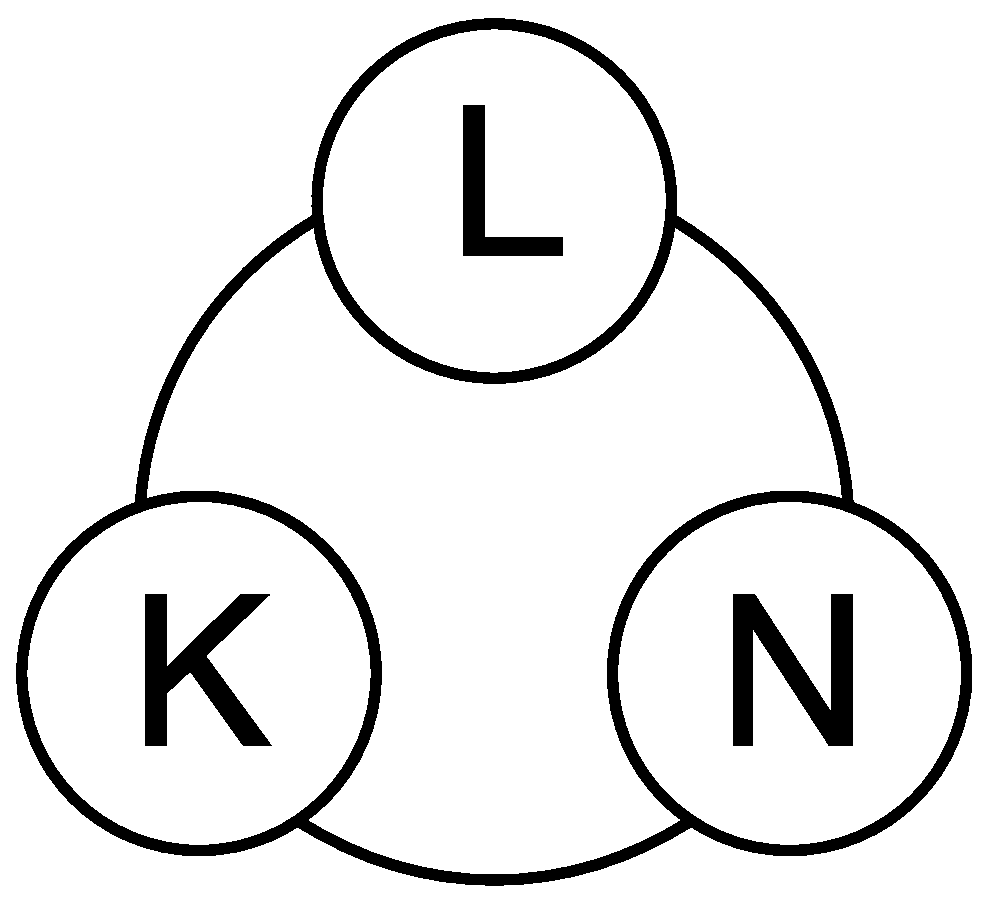
\includegraphics[width=4cm]{LKN_Logo_klein}
  \end{center}

\begin{center} {\sf\bf 
                               \Large  Technische Universität München
                                \smallskip

                               \Large Lehrstuhl für Kommunikationsnetze
                               \smallskip
                              }

                              {\sf \large Prof. Dr.-Ing. Wolfgang Kellerer} 
\end{center}  

\vspace{4cm}

\begin{center}
        {\bf\Huge Bachelor's Thesis} % Studienarbeit, Interdisziplinäres Projekt
\end{center}

\begin{center}
        \settowidth{\baselineskip}{0.4cm}
        {\LARGE 
        AoI-based Scheduling for Networked Control Systems over Gilbert-Elliot Channel 
        }
\end{center}

\vfill         
{\settowidth{\baselineskip}{0.2cm}
\large\begin{tabular}[l]{ll}
Author: & Henry He\\
Supervisor: & M.Sc. Onur Ayan\\
Begin: & 01. June 2020\\
End: & 19. October 2020
\end{tabular}}

%%%%%%%%%%%%%%%%%%%%%%%%%%%%%%%%%%%%%%%%%%%%%%%%%%%%%%%%%%%%

% MAIN PART:
% Independence and License statements
\thispagestyle{plain}


\vspace*{1cm}
With my signature below, I assert that the work in this thesis has been composed by myself independently and no source materials or aids other than those mentioned in the thesis have been used.



\vspace{2cm}

\hspace{1cm}\begin{tabular}{ccc}
\vspace{-0.3cm}München, 19.10.2020 	&\hspace{4cm} 		& \\
\rule{4.5cm}{0.4pt}					&					&\rule{4.5cm}{0.4pt}\\
Place, Date							&					& Signature			
\end{tabular}

           		






\vspace{4cm}
This work is licensed under the Creative Commons Attribution 3.0 Germany License. To view a copy of the license, visit http://creativecommons.org/licenses/by/3.0/de\\

Or\\

Send a letter to Creative Commons, 171 Second Street, Suite 300, San Francisco, California 94105, USA.

\vspace{2cm}



\hspace{1cm}\begin{tabular}{ccc}
\vspace{-0.3cm}München, 19.10.2020 	&\hspace{4cm} 		& \\
\rule{4.5cm}{0.4pt}					&					&\rule{4.5cm}{0.4pt}\\
Place, Date							&					& Signature	
\end{tabular}

% Abstract:
%\setlang{USenglish}
\thispagestyle{plain}

\section*{Abstract}
Many emerging applications to be supported by upcoming 5G networks can be seen
as Networked Control Systems (NCS), i.e., feedback control loops closed over a
communication network. Delay, limited network resources, time-varying channel
conditions are common network-induced challenges which can be tackled by a
scheduler granting medium access efficiently. Age-of-Information (AoI) is a
recently introduced network metric quantifying information freshness at a
receiving network node and is meant to serve as an interface between
communication network and application. AoI has generalized joint design in NCS,
where networking policies have to consider the underlying system dynamics of its
users. It has found successful use-cases in control-aware data scheduling. In
this work, we employ AoI to calculate penalty functions used to derive an
optimal control-aware scheduling strategy. We consider multiple, heterogeneous
NCS sharing a single wireless link with time-varying channel conditions governed
by the Gilbert-Elliot model. We have implemented a channel state dependent
scheduling algorithm and obtained its complexity. However, simulations have
shown that it is not scalable due to high computational costs. Furthermore, we
have investigated possible reasons behind inconsistent behavior of our
scheduling algorithm when simulated on different operating systems. The effect
occurs on Linux, Mac and Windows and results in the scheduler distributing
network resources differently, which leads to varying performance.

% Table of contents:
\tableofcontents  
% Introduction (Einleitung):
\chapter{Introduction}

% This chapter should give a short overview over the whole thesis. It should
% provide background information on the thesis topic, introduce the task
% definition and give a short outlook on the rest of the thesis. 

Development of the upcoming generation of communication networks are largely
driven by changing application demands. Instead of solely focusing on data rate
increase, these networks are envisioned to support machine-type-communications
(MTC) or machine-to-machine communications (M2M), transforming the current
``Internet of Information'' to a ``Internet of Things and Services''. Prominent
applications include vehicular networks, industrial automation, tele-robotics,
smart grids and cyber-physical systems \cite{murray2003future}. From a system
theoretical view, most of these emerging applications fall into the category of
\textit{Networked Control Systems} (NCS), i.e., feedback control loops closed
over a communication network. Each loop consists of a plant, a sensor, measuring
the plant's output, and the respective controller, reacting to the sensor's
data. \\
In a typical NCS scenario, multiple heterogenous NCSs share a wireless
communication medium and compete for network resources to transmit their latest
sensor measurements to the controllers. Medium access is granted by a
centralized scheduler that determines which subset of control loops are allowed
to send their up-to-date state information. In such a setting, the communication
system needs to satisfy different time-critical-requirements of the underlying
control loops, while dealing with problems inherent to the network, such as
random delays, packet losses and time varying channel conditions. These
shortcomings motivate \textit{control-aware} communication protocol design
incorporating prioritization and efficient scheduling of NCSs. Such schedulers
aim to mitigate these network induced challenges, which would otherwise result
in reduced precision of control actions and degraded control quality. Thus,
networking policies need to be designed in a joint fashion by using
\textit{cross-layer} metrics and considering detailed models of feedback control
loops. 

Clearly, the control performance of NCS, i.e., quality of control (QoC), is
tightly coupled with the service provided by the communication network. While
traditionally, performance of network systems are measured by means of delay,
jitter and throughput, these human-oriented metrics do not sufficiently capture
the QoC requirements of heterogeneous NCS applications. Hence, new cross-layer
metrics are needed in control-aware communication protocol design.
Age-of-Information (AoI) is such a relatively new metric that measures the
information freshness at the receiver monitoring a remote process
\cite{kaul2012real} and is used as a cross-layer metric in wireless medium
access protocol design. It is defined as the time elapsed since the generation
of the latest received information. As the name implies, AoI increases linearly
in time for all types of applications and drops upon receiving a new update. AoI
combines packet generation frequency, end-to-end delay, and packet loss in a
single metric. For instance, the absence of information increases AoI on the
controller side regardless of its cause: high delay, packet loss, or a low
information update frequency. As an interface between control application and
communication network, AoI has been widely adopted as an intermediate metric to
calculate control system metrics. 

% While such a setting allows control over large distances, wireless networks
% inevitably introduce random delays, packet losses and time varying channel
% conditions, degrading the control quality. As modern control theory is based on
% the assumption that information are transmitted along perfect communication
% channels, imperfections of the wireless channel or time-critical requirements of
% the underlying control loops impose challenges for both communication and
% control. 

\section*{Problem Statement}
In this work, we aim to develop an optimal scheduling policy addressing a
centralized wireless resource scheduling problem for NCS. We consider multiple
heterogenous feedback control loops sharing a wireless link with time-varying
channel conditions according to the Gilbert-Elliot Model. The deviation of the
real state from the estimated state on the receiver, i.e. controller, is taken
as performance metric. To provide optimal NCS behavior, we utilize AoI-based,
control dependent age-penalties and form scheduling decisions by means of
expected cost minimization. For a similar scenario, \cite{ayan2020aoi} has
proposed an online, centralized scheduling policy that is age-penalty optimal
for a finite horizon $H$. However, similar to most existing works, this solution
assumes a channel with independent and identically distributed (i.i.d) packet
loss. Wireless channels on the other hand are known to generate burst packet
losses/errors, meaning in reality packet losses tend to be correlated. One
simple model capturing correlated losses found in wireless fading channels is
the Gilbert-Elliot Model. We aim to extend the state-of-the-art by combining our
findings of the Gilbert-Elliot Channel Model with the said AoI-based Finite
Horizon scheduler.



% Text Body (Hauptteil)
% Could have multiple chaper-files, e.g.:
\chapter{Background}

In this chapter, all background necessary to understand the thesis are introduced. The level of detail is such that a colleague with similar background (no specialist!) is capable of understanding the contribution and impact of the thesis. A discussion of state-of-the-art solutions (e.g. literature research) is often helpful. Problems of the state-of-the-art are typically discussed and the contribution of the thesis is introduced in detail. 

\section{Related Work}

\section{Gilbert-Elliot Model}

In a wireless communication environment, channel errors are bursty, location
dependent, and mobility dependent. These are due to radio propagation
impairments such as shadowing and multipath fading, as well as interference from
neighboring systems and users. In addition, one must take into account that
users of a wireless network, do not perceive the same channel quality at all
times, where channel quality is considered high when its bit error rate (BER) is
low. Thus, there is one wireless channel (link) between each pair of spatially
distributed nodes (users). 

\begin{figure}[h]
  \centering
  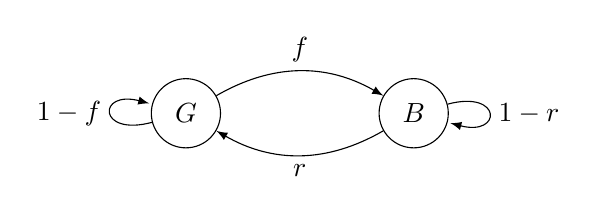
\begin{tikzpicture}[->,>=latex]
  % Create nodes
  \node[state] (G) {$G$};
  \node[state] (B) [right = 2cm of G] {$B$};

  % 
  \path (G) edge [loop left, left] node {$1-f$} (G);
  \path (B) edge [loop right, right] node {$1-r$} (B);
  \path (G) edge [bend left, above] node {$f$} (B);
  \path (B) edge [bend left, below] node {$r$} (G);
\end{tikzpicture}
 
  \caption{The Markov chain for the Gilbert-Elliot model}
  \label{fig:GE_FSM}
\end{figure}

In the literature, the time-varying quality of a bursty error wireless channel
is commonly modeled using the \textit{Gilbert–Elliot} model (GE)
\cite{gilbert1960capacity}
\cite{elliott1963estimates}. It is a widely used stochastic model for describing
bit error processes in transmisson channels, where errors are correlated. There
are several parameterizations of this model, but we will use the specific Markov
chain shown in Fig. \ref{fig:GE_FSM}. This model is a two-state homogenous
Markov chain where each of the two states corresponds to high or low channel
quality and is called good state $G$ or bad state $B$, respectively. Each of them may
generate errors as independent events at a state dependent error rate $p_G$ in
the good and $p_B$ in the bad state. As shown in \cite{hasslinger2008gilbert},
to apply the model in data loss processes, we consider the packet reception
process as a sequence of bits: 0 stands for a successful arrival
of a packet whereas 1 denotes a lost or corrupted packet.

Let $q_t$ denote the state at time $t$, the GE model is defined by the
transition matrix $\Pi$

\begin{equation*}
  \Pi = \left (\begin{array}{cc} 1-f & f \\ r & 1-r \end{array} \right) 
\end{equation*}
\begin{align*}
  f &= P(q_t = B \mid q_{t-1} = G) \qquad \textrm{failure rate} \\
  r &= P(q_t = G \mid q_{t-1} = B) \qquad \textrm{recovery rate}
\end{align*}

where $f\in(0,1)$ and $r\in(0,1)$ are the transition probabilty between states,
respectively. With these definitions, the stationary state probabilties of the
good state $\pi_G$ and $\pi_B$ exist and can be defined as follows:

\begin{equation}
  \pi_G = \frac{r}{f+r} \quad \textrm{and} \quad \pi_B = \frac{f}{f+r}
\end{equation}

The stationary state probabilties can be interpreted as the average percentage
of time, in which the channel is in good or bad state. Thus, the \textit{average
error probabilty} is obtained as:

\begin{equation}
  p_E = \pi_G p_G + \pi_B p_B
  \label{eq:avgLoss}
\end{equation}

Another important characteristic defined by the GE model is the mean sojourn
time, i.e., the average duration that the wirless channel stays in a state. In
common NCS scenarios, packet transmissions occur in discrete time slots. Hence,
the channel can only change its state in these time slots and the amount of time
spent in a state is a geometrically distributed random variable $\tau_G$ and
$\tau_B$. Given the state transition probabilties, the mean sojourn times are:

\begin{equation}
  T_G = \E[\tau_G] = \frac{1}{f} \quad \textrm{and} \quad T_B = \E[\tau_B] = \frac{1}{r}
\end{equation}

Table \ref{tab:sojournTime} summarizes sojourn times measurements performed
under different GE parameterizations. The measurements resembles the expected
statistical properties of a geometric distribution and confirms our mapping of
state transition probabilties to their corresponding mean sojourn time, which we
will term \textit{average coherence time} throughout the rest of the thesis.

\begin{table}[h]
  \begin{center}
  \begin{tabular}{|p{3.5cm}|c|c|c|c|}
  \hline 
  & \multicolumn{2}{|c|}{\textbf{Time in Good}} &
  \multicolumn{2}{|c|}{\textbf{Time in Bad}} \\
  \hline
  \textbf{Failure rate} $f$ / \textbf{Recovery rate} $r$ & \textbf{mean} & \textbf{std} & \textbf{mean}
  & \textbf{std}\\
  \hline \hline
  0.3 & 3.34 & 2.74 & 3.32 & 2.77 \\
  \hline 
  0.1 & 10.0 & 9.56 & 10.0 & 9.29 \\
  \hline 
  0.03 & 33.4 & 32.6 & 34.1 & 34.1 \\
  \hline 
  0.01 & 94.3 & 89.5 & 98.1 & 99.6 \\
  \hline 
  \end{tabular}
  \caption{Measurment of sojourn times for different transition probabilties. Note that the state transition
  probabilties are chosen symmetrically for this measurement, i.e. $f=r$}
  \label{tab:sojournTime}
  \end{center}
  \end{table}


\section{Dynamic Programming Algorithm}

Dynamic programming (DP) is both a mathematical optimization method and a
computer programming method. The method was developed by Richard Bellman in the
1950s and has found applications in numerous fields, from aerospace engineering
to economics. In the context of this thesis, DP is applied in solving a wireless
resource scheduling problem. We will first describe the principles of the DP
algorithm with a general decision problem. To this end, we formulate a broadly
applicable model of optimal control of a dynamic system over a finite number of
stages (a finite horizon). Detailed application of DP to our scheduling problem
will be given in chapter. 

As such, it resembles a general problem of decision under stochastic
uncertainty, which has two principal features. An underlying discrete-time
dynamic system and a \textit{cost function}. Solving the decision problem
entails in minimizing this cost function, subject to the system's dynamics.
Given a discrete-time dynamic system of the form

\begin{equation*}
  x_{k+1} = f_k(x_k, u_k, w_k), \quad k = 0,1,\dots,N-1,
\end{equation*}

where

\begin{table}[h]
  \centering
  \begin{tabular}{rl}
    $k \in$ & indexes discrete time, \\
    $x_k \in$  & is the system's state and summarizes past information, \\
    $u_k \in$ & is the control or decision variable to be selected at time $k$, \\
    $w_k \in$ & is a random paramter, also called distrubance or noise, \\
    $N$ & is the horizon or number of times control is applied, 
  \end{tabular}
\end{table}

and $f_k$ is a function that describes the system's dynamics. The dynamic system expresses the evolution of the system's state, under the
influence of decisions made at discrete instances of time. 

The cost function is additive over time in the sense that the cost incurred at
time $k$, denoted by $g_k(x_k, u_k, w_k)$, accumulates over time. The total cost
is

\begin{equation*}
  g_N(x_N) + \sum\limits_{k=0}^{N-1}{g_k(x_k, u_k, w_k)},
\end{equation*}

where $g_N(x_N)$ is the terminal cost incurred at the end of the process.
However, since randomness introduced is by $w_k$, the cost is generally a
random variable and cannot be easily optimized. Therefore the optimal control
problem is formulated as an minimization of the \textit{expected cost}

\begin{equation*}
  J
\end{equation*}

\chapter{Scenario and Problem Statement}

Suppose $N$ independent, linear time-invariant (LTI) control systems sharing a
wirless communication network. Each individual subsytem $i$ consists of a plant
$\plant$, a sensor $\sensor$, and a controller $\controller$ with an estimator
$\estimator$. Each sensor $\sensor$ samples the plant periodically and transmits
the latest state information to $\controller$. On the controller side,
$\estimator$ estimates periodically the current plant state based on the latest
received information. Estimated state is then used by $\controller$ to calculate
the next control input. We assume each controller-plant pair to be co-located
and hence connected through an ideal link while the sensor is operating remotely
over the shared wirless channel as illustrated in Fig. \ref{fig:scenario}.

\begin{figure}[h]
  \centering
  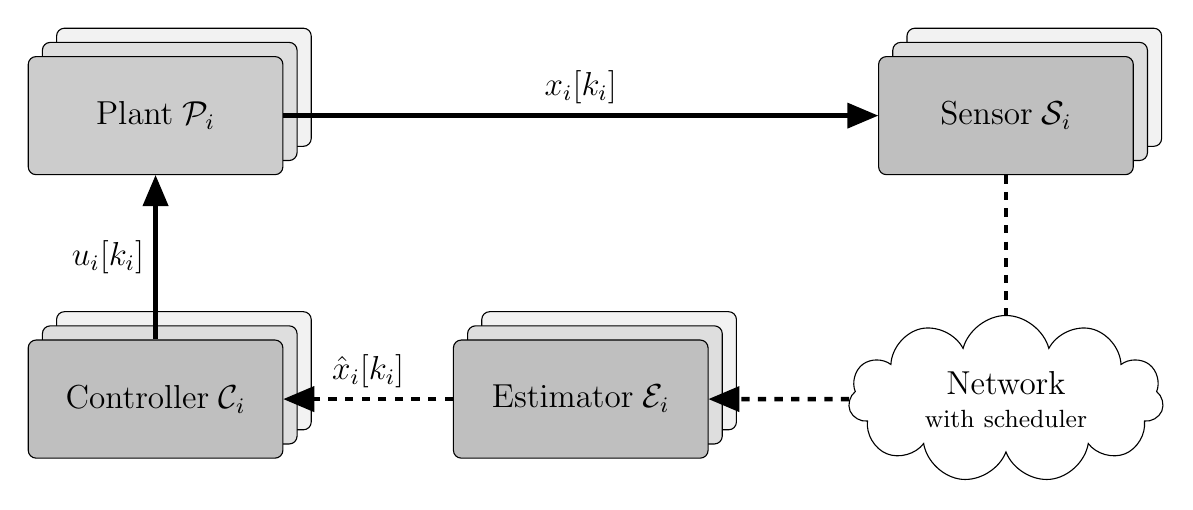
\begin{tikzpicture}[>=latex, scale=0.9]
  \node (plant) at (0.4,6.4) [draw,minimum width=2cm,minimum height=1.5cm, rounded corners=0.1cm, text width=3cm, align=center, fill=mylightestgray] {};
  
  \node (plant) at (0.2,6.2) [draw,minimum width=2cm,minimum height=1.5cm, rounded corners=0.1cm, text width=3cm, align=center, fill=mylightergray] {};
  
  % Plant
  \node (plant) at (0,6) [draw,minimum width=2cm,minimum height=1.5cm, rounded corners=0.1cm, text width=3cm, align=center, fill=mygray] {\large{Plant $\mathcal{P}_i$}};
  
  
  % Sensor 
  \node (sensor) at (12.4,6.4) [draw,minimum width=2cm,minimum height=1.5cm, rounded corners=0.1cm, text width=3cm, align=center, fill=mylightestgray] {};
  
  \node (sensor) at (12.2,6.2) [draw,minimum width=2cm,minimum height=1.5cm, rounded corners=0.1cm, text width=3cm, align=center, fill=mylightergray] {};
  
  \node (sensor) at (12,6) [draw,minimum width=2cm,minimum height=1.5cm, rounded corners=0.1cm, text width=3cm, align=center, fill=lightgray] {\large{Sensor $\mathcal{S}_i$}};
  
  %Estimator
  \node (estimator) at (6.4,2.4) [draw,minimum width=2cm,minimum height=1.5cm, rounded corners=0.1cm, text width=3cm, align=center, fill=mylightestgray] {\large{Estimator $\mathcal{E}_i$}};

  \node (estimator) at (6.2,2.2) [draw,minimum width=2cm,minimum height=1.5cm, rounded corners=0.1cm, text width=3cm, align=center, fill=mylightergray] {\large{Estimator $\mathcal{E}_i$}};

  \node (estimator) at (6,2) [draw,minimum width=2cm,minimum height=1.5cm, rounded corners=0.1cm, text width=3cm, align=center, fill=lightgray] {\large{Estimator $\mathcal{E}_i$}};


  % Controller
  \node (controller) at (0.4,2.4) [draw,minimum width=2cm,minimum height=1.5cm, rounded corners=0.1cm, text width=3cm, align=center, fill=mylightestgray] {};
  
  \node (controller) at (0.2,2.2) [draw,minimum width=2cm,minimum height=1.5cm, rounded corners=0.1cm, text width=3cm, align=center, fill=mylightergray] {};
  
  \node (controller) at (0,2) [draw,minimum width=2cm,minimum height=1.5cm, rounded corners=0.1cm, text width=3cm, align=center, fill=lightgray] {\large{Controller $\mathcal{C}_i$}};
  
  
  % Network Cloud
  \node[cloud, cloud puffs=11, cloud ignores aspect, minimum width=2cm, minimum height=1.5, text width=2.5cm, align=center, draw] (cloud) at (12, 2) {\large {Network \\} \small{with scheduler}};
  
  % C-to-P arrow
  \draw[arrows=-triangle 45,black, ultra thick] (controller.north) -- node[pos=0.5, left] {\large $u_i[k_i]$} (plant.south);
  
  % P-to-S arrow
  \draw[arrows=-triangle 45,black, ultra thick] (plant.east) -- node[pos=0.5, above] {\large $x_i[k_i]$} (sensor.west);
  
  % P-to-Cloud arrow
  \draw[black, dashed, ultra thick] (sensor.south) -- node[] {} (cloud.north);
  
  % Cloud-to-E arrow
  \draw[arrows=-triangle 45,black, dashed, ultra thick] (cloud.west) -- node[pos=0.5, above] {} (estimator.east);

  % E-to-C arrow
  \draw[arrows=-triangle 45,black, dashed, ultra thick] (estimator.west) -- node[pos=0.5, above] {\large $\hat{x}_i[k_i]$} (controller.east);
  
  \end{tikzpicture}

  \caption[Scheme of $N$ subsytems sharing a wirelss communication medium]{Considered scenario with $N$ heterogenous LTI networked control systems. Solid lines indicate ideal controller-to-plant and plant-to-sensor links. Sensor-to-contoller link is closed over a shared wireless channel. Medium access is granted centrally by a scheduler. Note that $k_i$ refers to the sampling period a sub-system $i$ is in.}
  \label{fig:scenario}
\end{figure}


\section{Network Model}
Time is divided into slots which is also the smallest time unit in our scenario.
We use $t \in \mathbb{N}$ All transmissions are managed by a centralized entity
called \textit{scheduler}.

\section{Age-of-Information Model}

\section{Control Model}

\section{Scheduling Problem Formulation} \label{sec:problem}

\chapter{Scheduler Design}

\chapter{Evaluation}
\section{Implementation}
Details regarding implementation and/or simulation are given in this chapter. The considered setup and the parameters used are introduced and discussed. Also, the general evaluation methods can be presented. (Note: Code should not be part of this chapter. If it makes sense to introduce it into the thesis, it should be placed in the appendix.)

\section{Results}
Results of the performed investigations are presented here. Interpretations for the observed effects are given and the impact of investigations is discussed. 

%  Conclusions (Zusammenfassung):
\chapter{Conclusion}

The thesis is concluded here. The considered problem is repeated. The
contribution of this work is highlighted and the results are recapitulated.
Remaining questions are stated and ideas for future work are expressed. 


\listoffigures
\listoftables

% Abbreviations (Abkürzungsverzeichnis):
\chapter*{Notation and Abbreviations}
% This chapter contains tables where all abbreviations and other notations like mathematical
% placeholders used in the thesis are listed.

\begin{tabular}{p{2cm} l} 
$\boldsymbol{v}^T$ & Transpose of vector $\boldsymbol{v}$\\
$\boldsymbol{M}^T$ & Transpose of matrix $\boldsymbol{M}$\\
$\tr(.)$ & Trace operator i.e. sum of all diagonal elements of a matrix\\
$\E[\mathit{X}]$ & Expected value of a random variable $\mathit{X}$\\
$\|\boldsymbol{v}\|$ & Euclidean norm of a vector $\boldsymbol{v}$ with $\|\boldsymbol{v}\|=\sqrt{\boldsymbol{v} ^T\boldsymbol{v}}$\\
$\mathcal{N}(\mu,\sigma^2)$ & Normal distribution with mean $\mu$ and standard deviation $\sigma$\\
$\mathcal{U}(a,b)$ & Uniform distribution with minimum and maximum values $a$ and $b$\\
$\Pr\left[A \mid B \right]$ & Occurrence probability of an event $A$ given $B$\\
$\mathbb{Z}^+$ & Set of positive integer numbers\\
$\mathbb{N}$ & Set of natural numbers\\
\end{tabular}
\vspace{1cm}

\hrule
\vspace{1cm}
  
\begin{tabular}{>{\bfseries}p{2cm} l}
AoI & Age-of-Information\\
BER & Bit Error Rate\\
DP & Dynamic Programming\\
FHS & Finite Horizon Scheduler\\
GE & Gilbert-Elliot\\
GES & Gilbert-Elliot Channel-aware Scheduler\\
i.i.d & independent and identically distributed\\
LTI & Linear Time-Invariant\\
MTC & Machine Type Communication\\
M2M & Machine-to-Machine\\
MSE & Mean Squared Error\\
NCS & Networked Control Systems\\
OS & Operating System\\
QoC & Quality of Control\\
VoI & Value-of-Information\\
w.r.t & with regards to\\
\end{tabular}


% References (Literaturverzeichnis):
% a) Style (with numbers: use unsrt):
\bibliographystyle{alpha}
% b) The File:
\bibliography{other/Bibliography}

% Appendix (Anhänge), could have multiple chaper-files:
\appendix
\chapter{}
The appendix may contain some listings of source code that has been used for simulations, extensive proofs or any other things that are strongly related to the thesis but not of immediate interest to the reader. 

%%%%%%%%%%%%%%%%%%%%%%%%%%%%%%%%%%%%%%%%%%%%%%%%%%%%%%%%%%%%


%%%%%%%%%%%%%%%%%%%%%%%%%%%%%%%%%%%%%%%%%%%%%%%%%%%%%%%%%%%%


%%%%%%%%%%%%%%%%%%%%%%%%%%%%%%%%%%%%%%%%%%%%%%%%%%%%%%%%%%%%
\end{document}
